\documentclass[10pt,aspectratio=169]{beamer}
\usefonttheme{professionalfonts}
\usepackage[utf8]{inputenc}
\usepackage{fontspec}
\usepackage{unicode-math}
\setsansfont{Fira Sans Light}
\setmathfont{Fira Math Regular}
% \usepackage{animate}
\usepackage{multimedia}
% \setmathfont{Fira Math Regular}
\title{\Large \bfseries Introduction to Logistic Regression}
\subtitle{CHE 358 Mock Lecture}
\author{Tian Tian}
\date{22 June 2023}
    

\begin{document}
    
\frame{\titlepage}


\begin{frame}
\frametitle{Perspective of Lecture}
\begin{enumerate}
\item The classification problem
\item Logistic regression vs linear regression
\item Fitting a logistic regression
\item Case study: Li-ion battery failure
\item Beyond logistic regression: neural networks
\end{enumerate}
\end{frame}

\begin{frame}
  \frametitle{Categorical Response Variables}

  Many real-world problems
  have \textbf{categorical} response variables instead of
  \textbf{continuous} ones:

  \begin{itemize}
    \item Diagnostics: 	is a patient \textbf{obese} or \textbf{not obese}
\item Decision:      	the valve A of reactor B be turned \textbf{on} or \textbf{off}
\item Data discretization:  \textbf{pass} or \textbf{fail} a material strength test
\item Describing types: \textbf{cubic}, \textbf{hexagonal}, \textbf{triclinic} lattices, etc.

\end{itemize}

\vspace{2em}

Categorical response variables differ from continuous variables:
\begin{itemize}
\item \textbf{Qualitative} rather than \textbf{quantitative}
\item May \textbf{not} have ordering
\item Distance between data points are usually \textbf{not meaningful}
\end{itemize}


\end{frame}

\begin{frame}
  \frametitle{The Classification Problem}

  Given:
  \begin{enumerate}
  \item Dataset: $\mathsf{D}$ with observations
    ${(X_{1}, y_{1}), (X_{2},y_{2}), \dots , (X_{n}, y_{n})}$
    
  \item Categorical response variable $y$: $y_{i} \in \mathsf{C}$, $\mathsf{C} = \{C_{1}, C_{2}, \dot, C_{k}\}$
  \end{enumerate}

  The model: $\mathsf{f}(X | \mathsf{D})$ that predicts the category of output.

  \vspace{2em}

  % \vfill
  \begin{columns}[T]
    \begin{column}{0.5\textwidth}
    What classification model will achieve:
    \begin{enumerate}
    \item Predict the categorical label
    \item Decision boundary for separation
    \item Probability of outcome
    \end{enumerate}
  \end{column}
  
\begin{column}{0.5\textwidth}
  \begin{figure}[t]
    \vspace{-2em}
     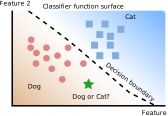
\includegraphics[width=0.98\textwidth]{images/classification_dog_cat.pdf}
    \end{figure}
\end{column}
  \end{columns}
  
\end{frame}

\begin{frame}
  \frametitle{Thought Experiment: the Cheater’s Coin}
  Imagine you’re a owner of a casino and wish to create a ``cheater's
  coin'' by varying the unbalanced weight distribution between its
  tails and heads. How can you improve the coin design based on your
  data?
  \vfill
  \begin{columns}[T]
    \begin{column}{0.20\textwidth}
      \begin{figure}[t]
        \includegraphics[width=\textwidth]{images/coin.pdf}
      \end{figure}
    \end{column}
    \begin{column}{0.75\textwidth}
      % \movie[loop]{}{scripts/animation.mp4}
      % \begin{figure}[t]
        % \animategraphics[width=\textwidth]{30}{scripts/animation-}{}{}
        % \includegraphics[width=\textwidth]{animation.gif}
      % \end{figure}
    \end{column}
  \end{columns}

\end{frame}
    
    
    
\end{document}
